\section{Tests and Test Status} \label{sec:testing}
Based roughly on \secref{sec:definition} there is a section here for each test we perform.
We consider since ComCam will not go on sky readiness may be demonstrated using AuxTel and/or Startracker data.

Any notebooks used for testing this will be in the notebook folder of the github repo containing this document.

\subsection{Data transferred and ingested in butler and access to data}
For a given observing day, verify after the end of the day that each raw image (identified by sequence number and detector) is available in the \texttt{/repo/embargo} Butler repository by retrieving it from both a development node (\texttt{rubin-devl}) and the USDF RSP (notebook and terminal).
Measure the delays between completion of readout for each image and the ingestion time recorded in the Butler Registry.
Verify that the 95th(TBD) percentile is less than 1 minute(TBD).

\textbf{This has been successfully.}

\subsubsection{Test execution}
\paragraph{Summit}
In the repo of this document \texttt{RTN-053-summit.ipynb} (\secref{sec:summitnb}) give the count of raws for a given night and lists detector and exposureid for the first and last.

\begin{lstlisting}
There are 592 raw in collection: ['LATISS/raw/all'] in: /repo/embargo for exposure.day_obs = 20230511
0 2023051100001
0 2023051100599
\end{lstlisting}

\paragraph{USDF}
In the repo of this document \texttt{RTN-053-USDF.ipynb} (\secref{sec:usdfnb}) gives the count of raws for the same night and lists detector and exposureid for the first and last.

\begin{lstlisting}
There are 592 raw in collection: ['LATISS/raw/all'] in: /repo/embargo for exposure.day_obs = 20230511
0 2023051100001
0 2023051100599
\end{lstlisting}

\paragraph {Ingest} \label{sec:ingest}
Also in the USDF notebook we get the ingest time and subtract the shutter close time to calculate the
delay to ingest.
\begin{lstlisting}
Got Metadata for 592 exposures
The min time was 0.19347863333343263 max time was 0.5866245333332909 minutes
Time between shutter close and ingest mean:0.23482382218469838, std:0.018058551157743862, var:0.0003261112699168522 minutes
\end{lstlisting}

\subsection{LFA replication to USDF }
Sample LargeFileObjectAvailable events from the USDF EFD (which will be verified as corresponding to the Summit EFD below).
Retrieve the corresponding LFA objects from the USDF LFA object store.

\textbf{This has been successful.}
\subsubsection{Test execution}
In the same notebooks  listed earlier there is a section 3.2

\paragraph{Summit} for given topic list large files on given day.
\begin{lstlisting}
Got 173 Large files available since 2023-04-20 at summit
\end{lstlisting}

\paragraph{USDF} check same topic same day in USDF.
\begin{lstlisting}
Got 173 Large files available since 2023-04-20 at USDF
result[168] https://s3.cp.lsst.org/rubinobs-lfa-cp/Electrometer:201/fits/2023/05/02/Electrometer:201_fits_2023-05-03T01:57:36.248.fits
Access s3://rubin:rubinobs-lfa-cp/Electrometer:201/fits/2023/05/02/Electrometer:201_fits_2023-05-03T01:57:36.248.fits
Object is 8640 bytes. b'SIMPLE  =                    T / conforms to FITS standard                      '
result[51] https://s3.cp.lsst.org/rubinobs-lfa-cp/Electrometer:201/fits/2023/05/02/Electrometer:201_fits_2023-05-02T23:45:47.304.fits
Access s3://rubin:rubinobs-lfa-cp/Electrometer:201/fits/2023/05/02/Electrometer:201_fits_2023-05-02T23:45:47.304.fits
Object is 8640 bytes. b'SIMPLE  =                    T / conforms to FITS standard                      '
result[73] https://s3.cp.lsst.org/rubinobs-lfa-cp/Electrometer:201/fits/2023/05/02/Electrometer:201_fits_2023-05-03T00:11:00.247.fits
Access s3://rubin:rubinobs-lfa-cp/Electrometer:201/fits/2023/05/02/Electrometer:201_fits_2023-05-03T00:11:00.247.fits
Object is 8640 bytes. b'SIMPLE  =                    T / conforms to FITS standard                      '
result[47] https://s3.cp.lsst.org/rubinobs-lfa-cp/Electrometer:201/fits/2023/05/02/Electrometer:201_fits_2023-05-02T23:41:17.827.fits
Access s3://rubin:rubinobs-lfa-cp/Electrometer:201/fits/2023/05/02/Electrometer:201_fits_2023-05-02T23:41:17.827.fits
Object is 8640 bytes. b'SIMPLE  =                    T / conforms to FITS standard                      '
result[121] https://s3.cp.lsst.org/rubinobs-lfa-cp/Electrometer:201/fits/2023/05/02/Electrometer:201_fits_2023-05-03T01:05:01.560.fits
Access s3://rubin:rubinobs-lfa-cp/Electrometer:201/fits/2023/05/02/Electrometer:201_fits_2023-05-03T01:05:01.560.fits
Object is 8640 bytes. b'SIMPLE  =                    T / conforms to FITS standard
\end{lstlisting}

\subsection{Automated prompt processing}
Verify that images taken with the ScriptQueue that have nextVisit events issued can be processed by a pipeline.
The pipeline will execute at least one step of single-frame instrument signature removal.
Verification will consist of retrieving the data products from the \texttt{/repo/embargo} Butler repository.

\textbf{This has been successful.}
\subsubsection{Test execution}
In the USDF notebook we query to Raws for a given night and also the prompt output collection.
Here we see  25 processed images of some 40 take in the evening.

\begin{lstlisting}
There are 655 raw in collection: ['LATISS/raw/all'] in: /repo/embargo for exposure.day_obs = 20230523
There are 25 calexp in collection: ['LATISS/prompt/output-2023-05-24/ApPipe/prompt-proto-service-00026'] in: /repo/embargo
\end{lstlisting}

As we did in \secref{sec:ingest} we can look at the shouter close time of the exposure which was used to make the calibrated image in prompt processing and the ingest of the processed image.
This gives an indication of prompt processing time.
\begin{lstlisting}
Time between shutter close and prompt mean:0.33115575866669145, std:0.20838310327912998, var:0.043423517732240555 minutes
The min time was 0.19349045000003784 max time was 0.9423351500001687 minutes for the 25 images
\end{lstlisting}


\subsection{EFD data available }
Choose at least 5 EFD topics at random from those available at the Summit.
Choose at least 20 messages per topic from those available at the Summit, including 10 from the previous observing day and 10 from past history.
Verify that all 100 messages are present in the USDF EFD.

\textbf{This has been successful.}

Choose 5 more topics that have graphs in the Summit Chronograf. Verify that the graph
shown for each topic for a specified time range is the same as that displayed by the USDF
Chronograf

\textbf{This has been successful - see \secref{sec:chrono}.}

\subsubsection{Test execution}

\paragraph{Summit} \label{sec:efdsummit}
In the repo of this document \texttt{RTN-053-summit.ipynb} (\secref{sec:summitnb})  section 3.4
selects some 10s of minutes of data from random topics from the same observing run above and from a day earlier in the month.
The results are stored in files and compared to the same  queries at USDF.

This is the output from the test run:

\begin{lstlisting}
lsst.sal.ATPtg.mountPositions had 29 messages
lsst.sal.ATPtg.mountPositions had 29 older messages
lsst.sal.MTAirCompressor.analogData had 46 messages
lsst.sal.MTAirCompressor.analogData had 46 older messages
lsst.sal.MTMount.elevationDrives had 456 messages
lsst.sal.GIS.logevent_heartbeat had 30 messages
lsst.sal.GIS.logevent_heartbeat had 30 older messages
lsst.sal.ESS.lightningStrikeStatus had 30 older messages
Random selection of five 'summit' topics ['lsst.sal.ATPtg.mountPositions',
'lsst.sal.MTAirCompressor.analogData', 'lsst.sal.MTMount.elevationDrives',
'lsst.sal.GIS.logevent_heartbeat'] with messages on 2023-04-20
Random selection of five 'summit' older topics ['lsst.sal.ATPtg.mountPositions',
'lsst.sal.MTAirCompressor.analogData', 'lsst.sal.GIS.logevent_heartbeat',
'lsst.sal.ESS.lightningStrikeStatus'] with messages on 2023-05-02
\end{lstlisting}

\paragraph{USDF}
In the repo of this document \texttt{RTN-053-USDF.ipynb} (\secref{sec:usdfnb})  section 3.4
loads the files mentioned in \secref{sec:efdsummit} and compare them:

\begin{lstlisting}
lsst.sal.ATPtg.mountPositions had 29 messages - summit had 29
lsst.sal.MTAirCompressor.analogData had 46 messages - summit had 46
lsst.sal.MTMount.elevationDrives had 456 messages - summit had 456
lsst.sal.GIS.logevent_heartbeat had 30 messages - summit had 30
Older messages
lsst.sal.ATPtg.mountPositions had 29 messages - summit had 29
lsst.sal.MTAirCompressor.analogData had 46 messages - summit had 46
lsst.sal.GIS.logevent_heartbeat had 30 messages - summit had 30
lsst.sal.ESS.lightningStrikeStatus had 30 messages - summit had 30
\end{lstlisting}

\paragraph{Chronograph - Summit and USDF} \label{sec:chrono}

\begin{figure}
\centering
\begin{subfigure}{.5\textwidth}
  \centering
  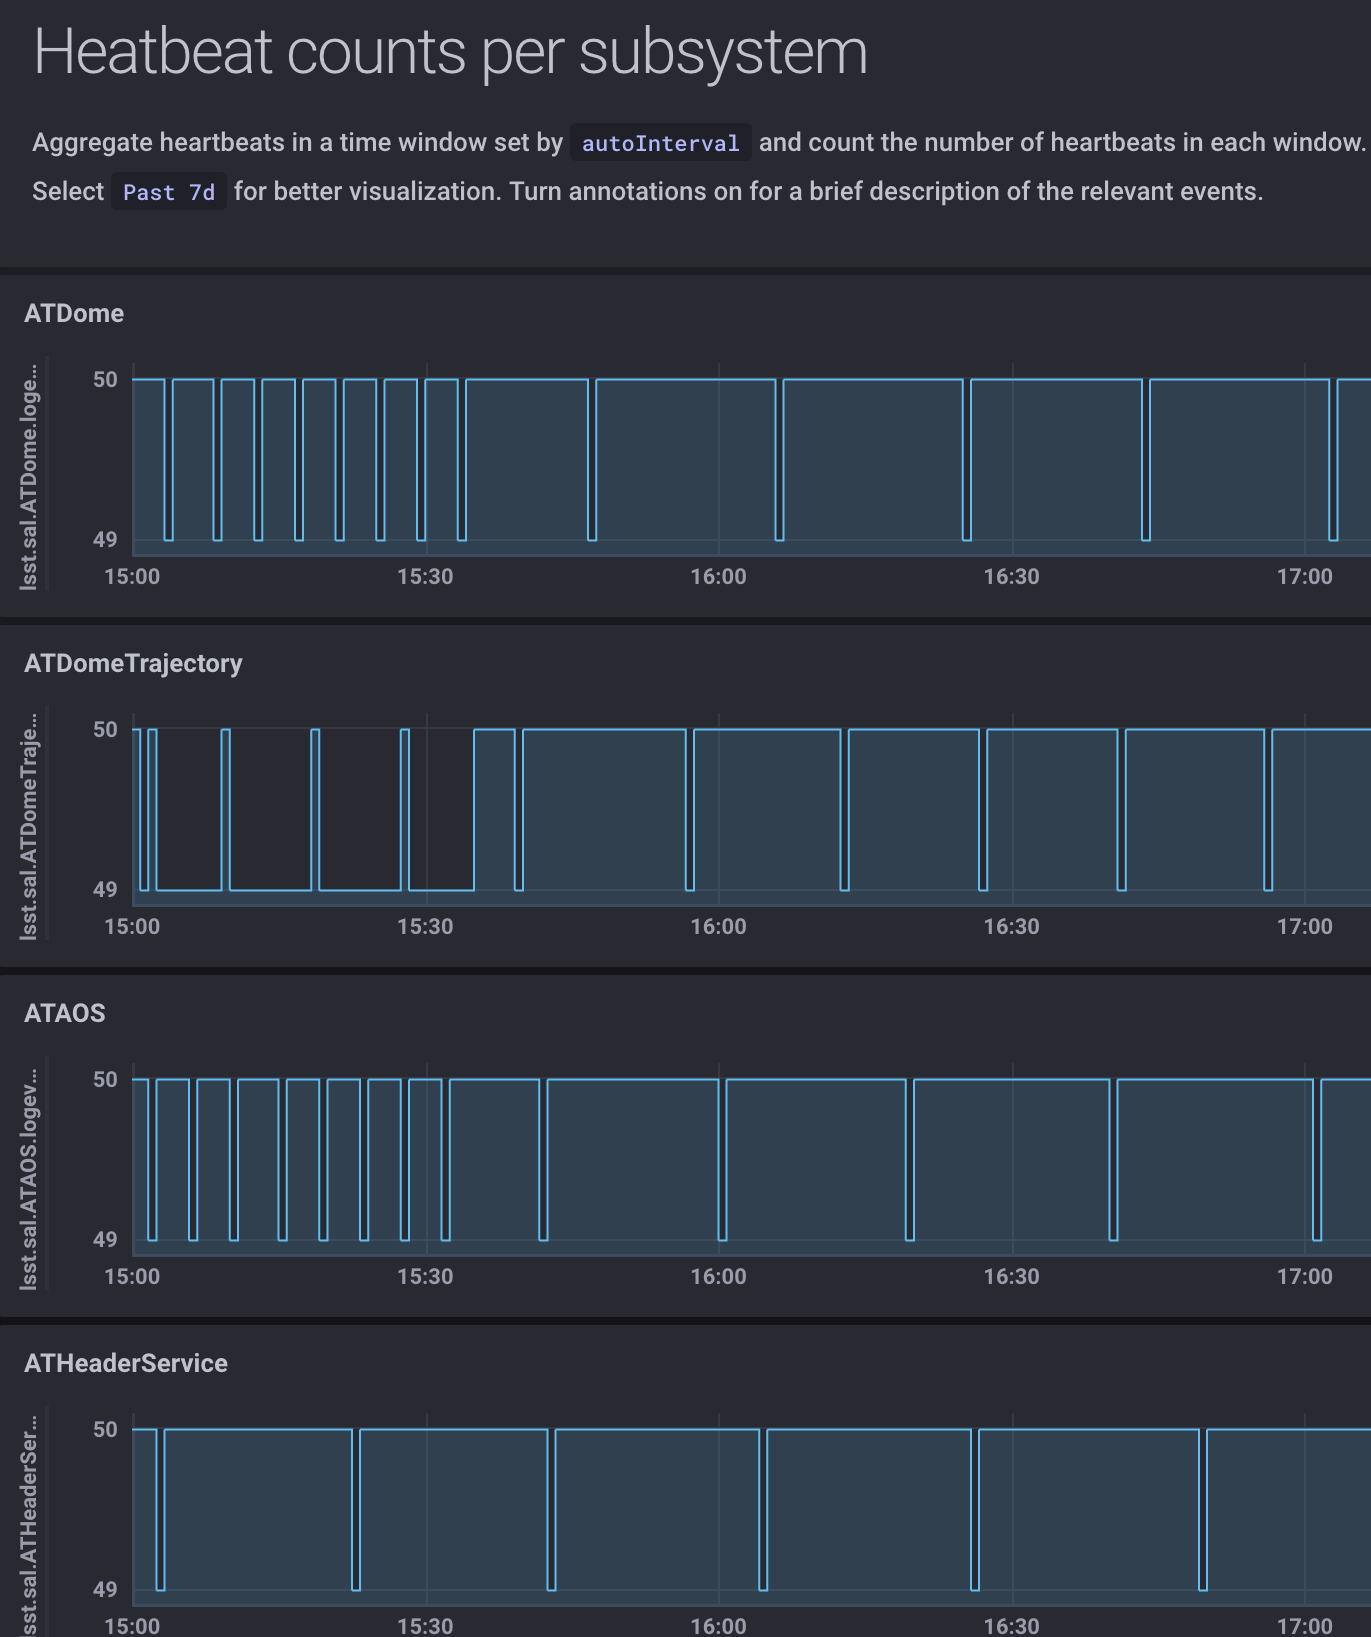
\includegraphics[height=4in]{images/Summit_1.png}
  \caption{Summit Chronograf 03-10-2023}
  \label{fig:sub1}
\end{subfigure}%
\begin{subfigure}{.5\textwidth}
  \centering
  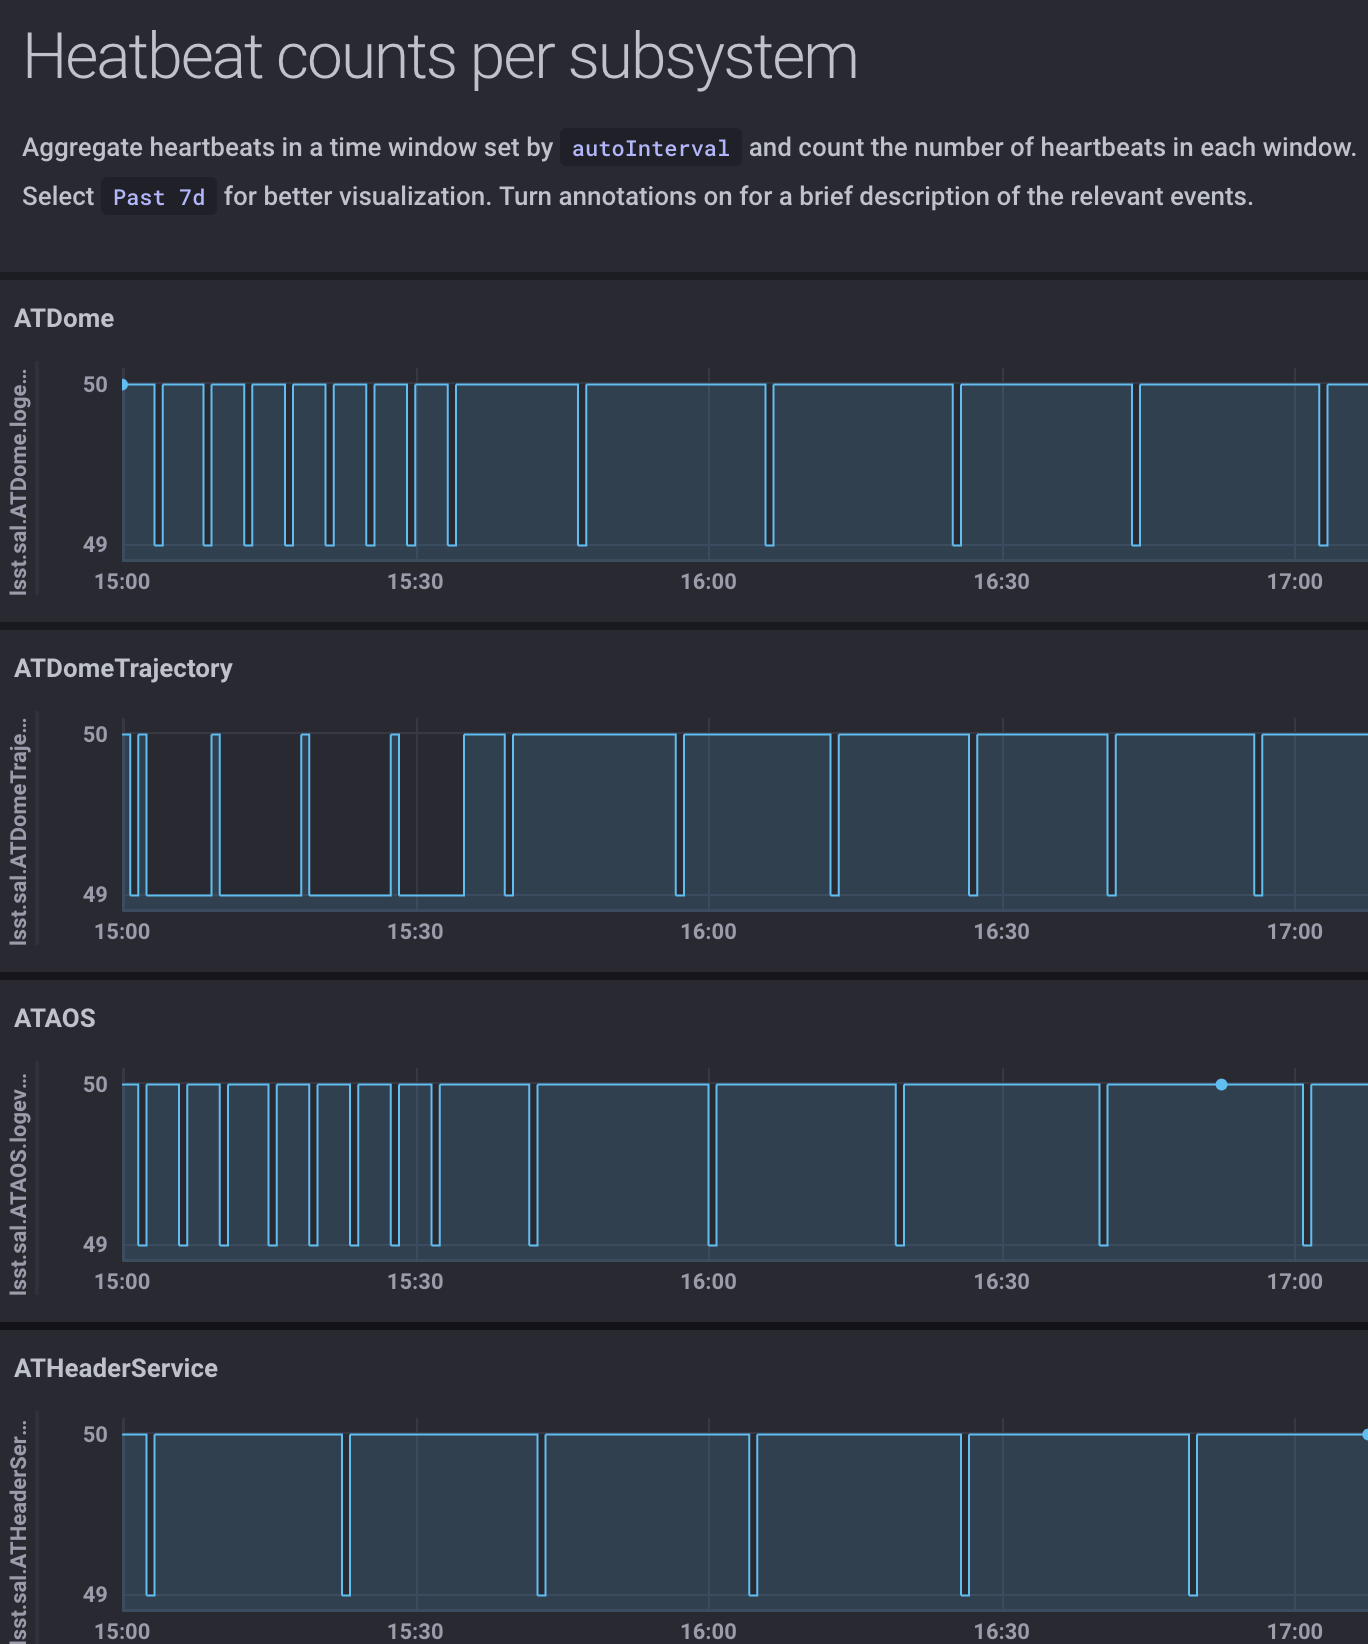
\includegraphics[height=4in]{images/USDF_1.png}
  \caption{USDF Chronograf 03-10-2023}
  \label{fig:sub2}
\end{subfigure}
\label{fig:image1}
\end{figure}
\setstretch{0.25}
Heartbeat Metrics compared between Summit and USDF Chronograf:
\begin{itemize}
  \item ATDome
  \item ATDome Trajectory
  \item ATAOS
  \item ATHeaderService
\end{itemize}

\newpage
\begin{figure}
\centering
\begin{subfigure}{.5\textwidth}
  \centering
  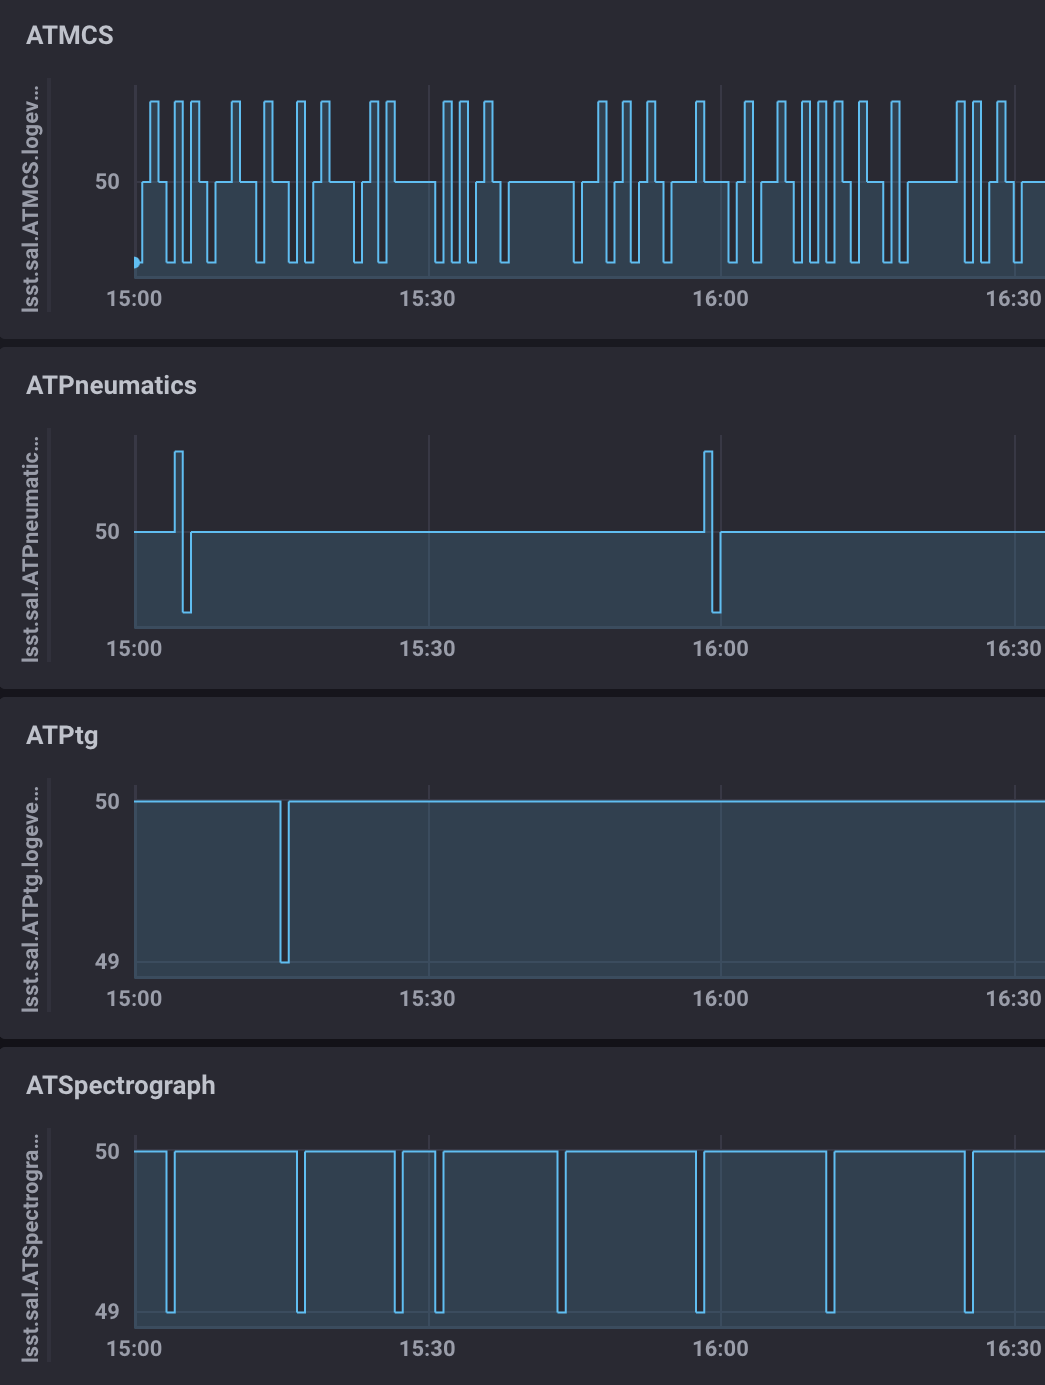
\includegraphics[height=4in]{images/Summit_2.png}
  \caption{Summit Chronograf 03-10-2023}
  \label{fig:sub3}
\end{subfigure}%
\begin{subfigure}{.5\textwidth}
  \centering
  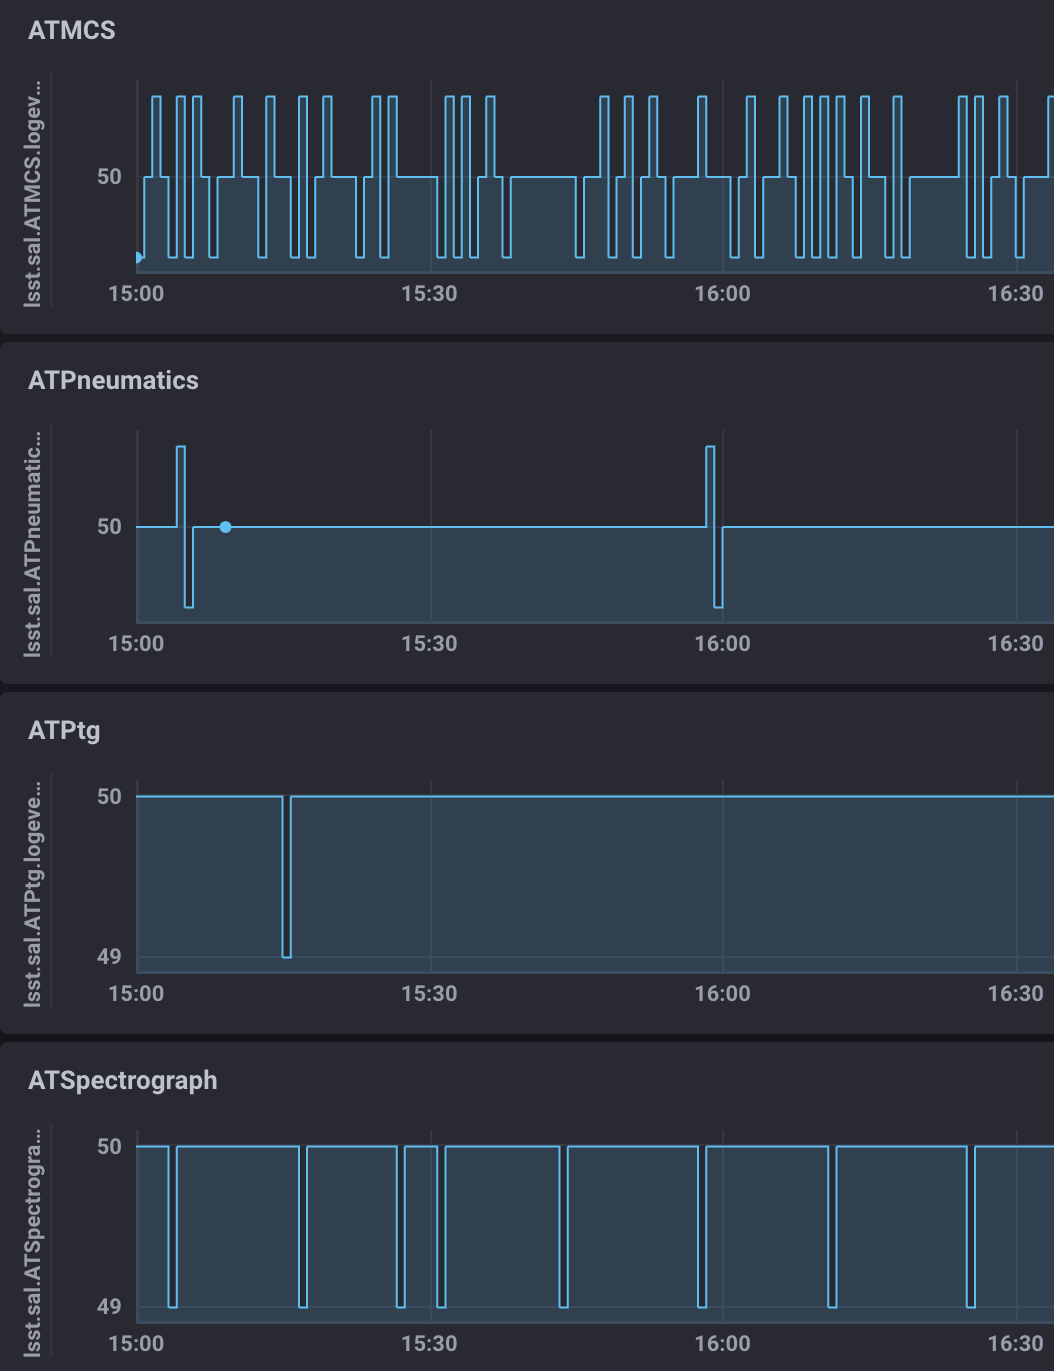
\includegraphics[height=4in]{images/USDF_2.png}
  \caption{USDF Chronograf 03-10-2023}
  \label{fig:sub4}
\end{subfigure}
\label{fig:image2}
\end{figure}
Heartbeat Metrics compared between Summit and USDF Chronograf:
\begin{itemize}
  \item ATMCS
  \item ATPneumatics
  \item ATPtg
  \item ATSpectrograph
\end{itemize}

\newpage
\begin{figure}
\centering
\begin{subfigure}{.5\textwidth}
  \centering
  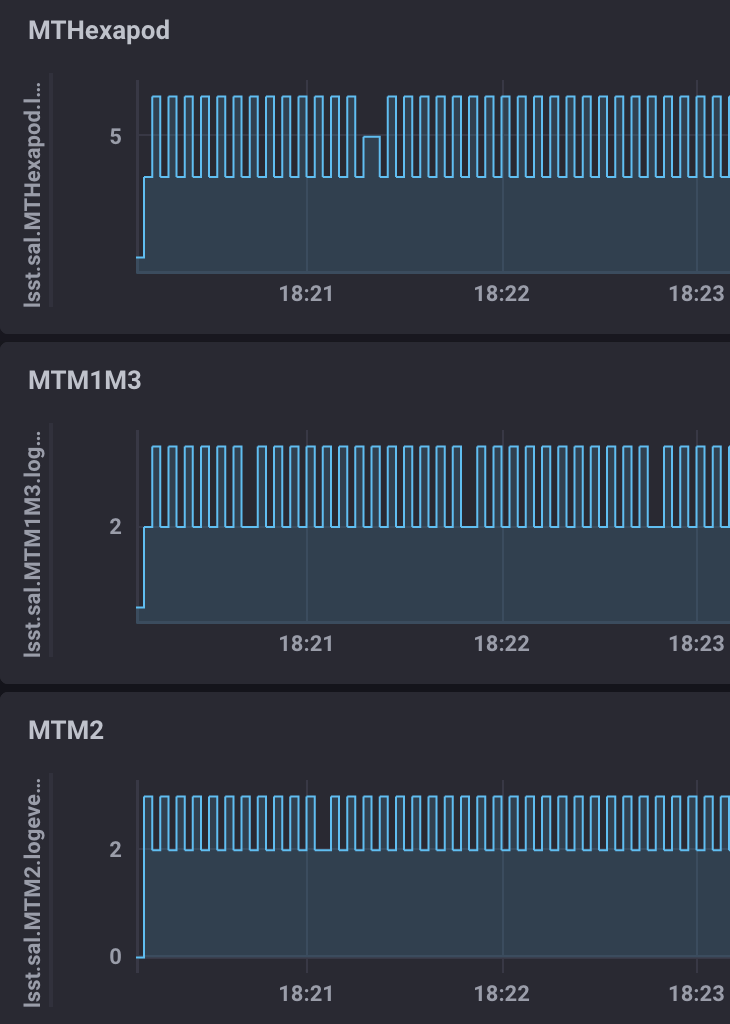
\includegraphics[height=4in]{images/Summit_3.png}
  \caption{Summit Chronograf 03-10-2023}
  \label{fig:sub5}
\end{subfigure}%
\begin{subfigure}{.5\textwidth}
  \centering
  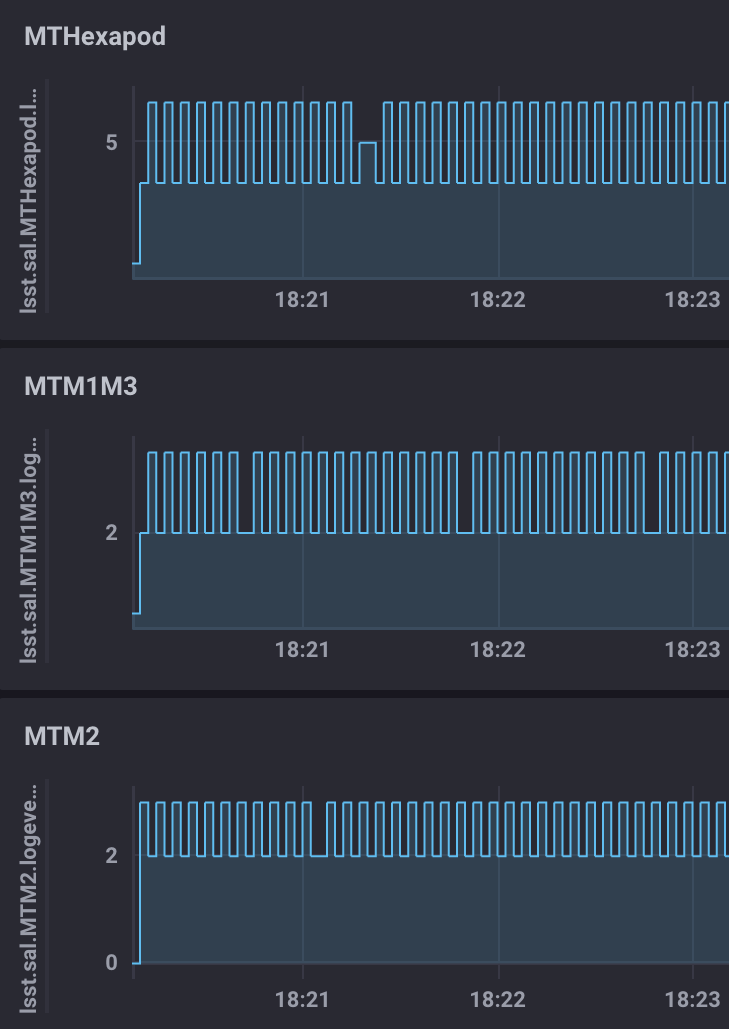
\includegraphics[height=4in]{images/USDF_3.png}
  \caption{USDF Chronograf 03-10-2023}
  \label{fig:sub6}
\end{subfigure}
\label{fig:image3}
\end{figure}
Heartbeat Metrics compared between Summit and USDF Chronograf:
\begin{itemize}
  \item MTHexapod
  \item MTM1M3
  \item MTM2
\end{itemize}

